\documentclass[12pt]{article}

\usepackage{graphicx}

\usepackage{fullpage}

\usepackage{amsmath}
\usepackage{xspace}
\newcommand{\transpose}[1]{\ensuremath{{#1}^\mathsf{T}}}
\newcommand{\JtJ}{\ensuremath{\transpose{J}\!J}\xspace}

\usepackage{url}

\usepackage[colorlinks,linkcolor=blue,citecolor=blue,urlcolor=blue]{hyperref}
\hypersetup{
bookmarksnumbered,
pdfpagemode=UseOutlines,
breaklinks=true,
}
\usepackage[figure]{hypcap}

\usepackage{listings}
\lstset{
basicstyle=\tt,
language=Python,
showstringspaces=False,
captionpos=b,
belowskip=0pt
}
\newcommand{\py}[1]{\lstinline[language=Python, showstringspaces=False]@#1@}
\newcommand{\shell}[1]{\lstinline[language=csh, showstringspaces=False]!#1!}
\newcommand{\ccode}[1]{\lstinline[language=C, showstringspaces=False]!#1!}

\newcommand{\filename}[1]{\texttt{#1}}

\sloppy %Prevent lines from running off edge of text

\begin{document}
\title{SloppyCell User Documentation\\
\large$Revision$}
\maketitle
\tableofcontents
\clearpage

Welcome to SloppyCell!

SloppyCell is a software environment for building and analyzing computational models of many-parameter complex systems.
To date, our focus has been on biochemical network models based on the Systems Biology Markup Language (SBML)~\cite{bib:Hucka2003}.
Many of the techniques and much of the code is, however, applicable to other types of models.

SloppyCell's goal is to provide a flexible environment that facilitates interactive exploratory model development while also remaining efficient for computation-intensive analyses.
This goal is facilitated by our use of the computing language Python (\url{http://www.python.org}) for both writing and driving SloppyCell.
SloppyCell scripts are Python programs, but please don't let that frighten you.
Python has proved easy to learn and there are numerous tutorials (e.g. \url{http://wiki.python.org/moin/BeginnersGuide}) and useful books~\cite{bib:Lutz2003}.
An excellent introduction to Python in the context of scientific computing is the May/June issue of Computing in Science and Engineering.

SloppyCell's development has been driven by the research interests of the Sethna group. For examples of the types of analysis we do, see our papers~\cite{bib:Brown2003a, bib:Brown2004, bib:Frederiksen2004, bib:Waterfall2006, bib:Casey2007, bib:Gutenkunst2007, bib:Gutenkunst2007a, bib:GutenkunstPhD}.

This document opens begins with an example application, followed by a high-level overview of SloppyCell's architecture.
We then delve into additional features and installation (Section~\ref{sec:user:install}), and we close with some troubleshooting.

Note: If you are using a binary installer, you will still want to download the source distribution (as described in Section~\ref{sec:test}) so that you will have access to the \shell{Example} and \shell{Doc} directories.

\section{JAK-STAT Example\label{sec:user:example}}

Here we consider an example application using the JAK-STAT model of Swameye et al.~\cite{bib:Swameye2003}, which was also used as an example by the SBML Parameter Estimation Toolkit (SBML-PET)~\cite{bib:Zi2006}.

\lstinputlisting[float,  basicstyle=\scriptsize, label=lst:user:example, numbers=left,  stepnumber=5, escapeinside={(@}{@)},
caption={[Example SloppyCell script for the JAK-STAT model] This script reproduces some of the results from~\cite{bib:Gutenkunst2008}. For detailed comments see Section~\ref{sec:user:example}.}
]{../../Example/JAK-STAT/run_JAK.py}

Using the script shown in Listing~\ref{sec:user:example}, we'll fit the model, build an ensemble, and then estimate some prediction uncertainties, reproducing most of the Figure from~\cite{bib:Gutenkunst2008}.
(This script is also found in the \shell{Example/JAK-STAT} directory of the SloppyCell source distribution.)
Some of the concepts may be a little subtle, so don't be afraid to turn to any section in the Overview and come back here.

Lines~\ref{code:import_start} through~\ref{code:import_end} \py{import} code from the Python packages we'll use this session: matplotlib, SciPy, and SloppyCell.

On line~\ref{code:SBML_import} we load the model network from the SBML file.
(Note that this file has been modified from the one included with SBML-PET to fix some bugs in it and to define the species \py{'data1'} and \py{'data2'} which correspond to the measurements we'll fit.)
Given the space constraints for listings here, the \py{Experiment} object is defined in another file, which we \py{import} on line~\ref{code:import_expt}.
We use that \py{Experiment}, along with our previously created \py{Network}, to create the \py{Model} object on the following line.

Our initial parameters are defined as a \py{KeyedList} starting on line~\ref{code:params}.
We could have specified them as a simple \py{list}, without the names, but we find things are much clearer when the names are visible as well.

A couple of priors need to be defined to keep model parameters from drifting too far.
The prior on \py{'r3'} (line~\ref{code:prior_start}) constrains it (within 95\% probability) to lie between $10^{-4}$ and $10^{4}$, while the prior on \py{'tao'} constrains it to lie between 1 and~16.

\begin{figure}
\begin{center}
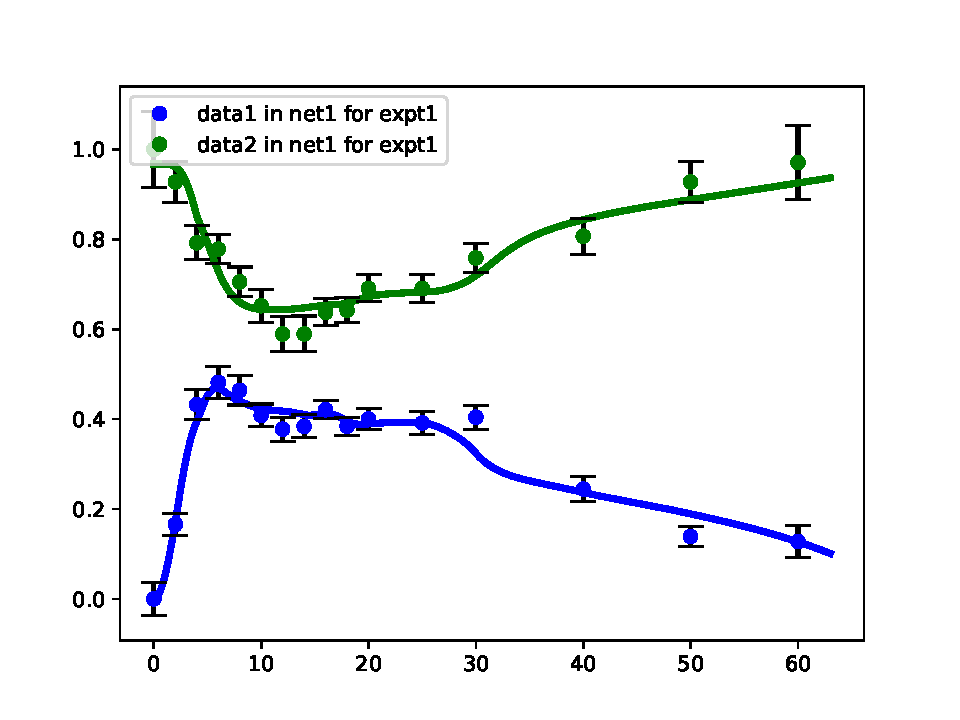
\includegraphics[width=3in]{../../Example/JAK-STAT/model_results}
\end{center}
\caption[Optimal fit for JAK-STAT example]{Plotted is the optimal fit for our example model, generated using \py{Plotting.plot_model_results(m)} in Listing~\ref{lst:user:example}.\label{fig:user:model_results}}
\end{figure}

The initial cost is about 560, which is very high given that we only have 32 data points.
Thus we run several iterations of Levenberg-Marquardt on line~\ref{code:lm_opt}.
(We limit the number of iterations here merely for expediency. This number gets us very close to the actual minimum.)
The final cost should be about 18.2. For a perfectly fitting model, we expect a cost of 1/2 the number of data points, so this cost indicates a good fit.
On line~\ref{code:plot_results} we generate Figure~\ref{fig:user:model_results}, which compares our best fit with the data.

Our group's philosophy is, however, not to trust solely in the best fit, so we'd like to build an ensemble of parameters.
Before we can build an ensemble, we need to build a matrix to guide the sampling.
Here we use the \JtJ approximation to the Hessian, which we calculate on lines~\ref{code:j_calc} and~\ref{code:jtj}.
(As an aside, the eigenvalues and eigenvectors of this \JtJ are `sloppy', as with the models discussed in~\cite{bib:Brown2003a, bib:Waterfall2006, bib:Gutenkunst2007}.)

On line~\ref{code:ens_gen} we build a parameter ensemble.
We only build a 7500 step ensemble because the model is quite small and well-constrained; with 5 parameters the correlation time should be only about 25 steps.
Also, we cast the \py{params} \py{KeyedList} to an array in the call; this makes our returned \py{ens} be composed of arrays rather than \py{KeyedList}s, which is more memory efficient.
Calculating a 7500 member ensemble for this model takes approximately 15 minutes on a modern PC.
On line~\ref{code:prune} we prune the ensemble; using slicing notation to take every 25th element (25 being the correlation time).
We also convert to an array, so that we can use the more powerful slice syntax of arrays.

\begin{figure}
\begin{center}
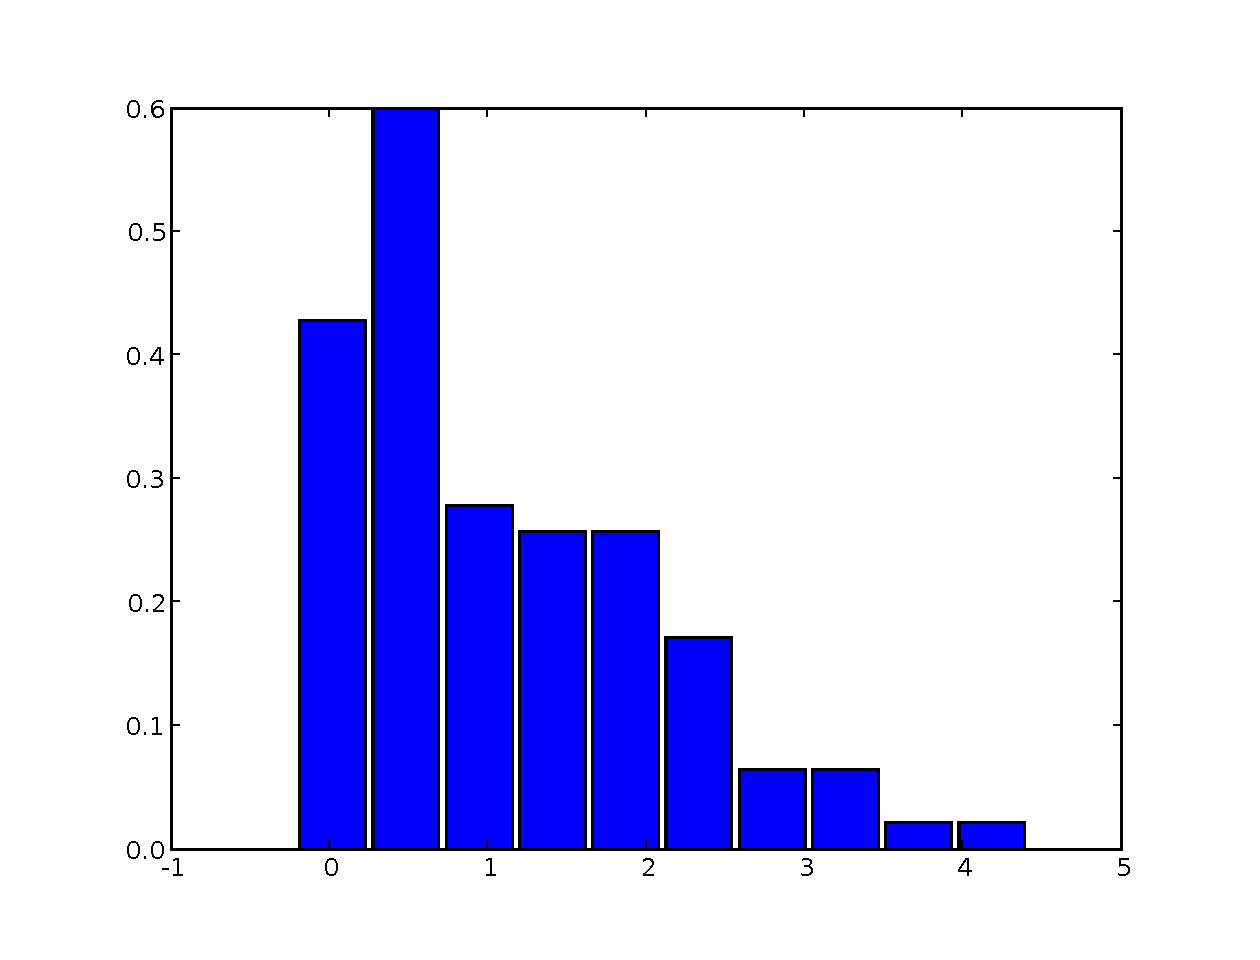
\includegraphics[width=3in]{../../Example/JAK-STAT/hist}
\end{center}
\caption[Histogram of $\log$ \py{'r3'} for the JAK-STAT model]{Shown is a histogram of $\log$ \py{'r3'} for the JAK-STAT ensemble. Note that the value of \py{'r3'} is bounded from below at about $10^0$, but the upper end is only bounded by the prior.\label{fig:user:hist}}
\end{figure}

What does the ensemble actually look like?
On line~\ref{code:hist}, we use matplotlib's \py{hist} function to build a histogram of the logarithm of \py{'r3'} over the ensemble.
The result is shown in figure~\ref{fig:user:hist}.
Note that the upper bound on \py{'r3'} is set by the prior we added, while the lower bound is constrained by fitting the data.

\begin{figure}
\begin{center}
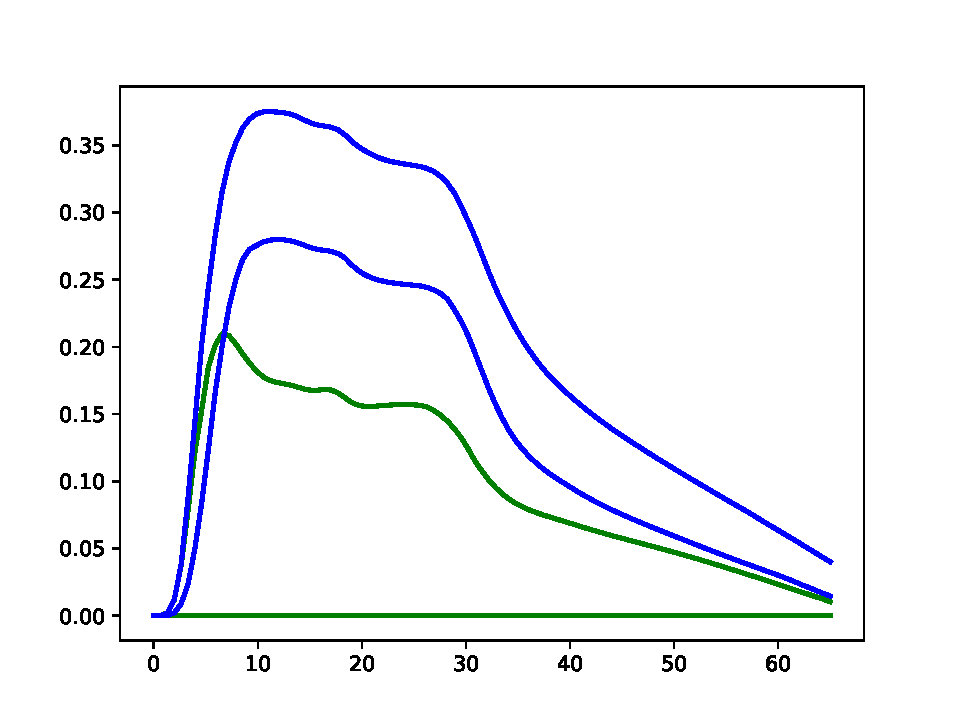
\includegraphics[width=3in]{../../Example/JAK-STAT/uncerts}
\end{center}
\caption[Prediction uncertainties for the JAK-STAT model]{In green is the 95\% uncertainty bound on cytoplasmic dimers, while blue is the 95\% bound on nuclear dimers, given the model and data that have been fit.\label{fig:user:uncerts}}
\end{figure}

Once we have our ensemble, we can make some predictions.
On line~\ref{code:ens_trajs} we calculate trajectories for \py{net} over our pruned ensemble, and on the following line we generate \py{lower} and \py{upper} trajectories that bound the central 95\% of the values for each variable.
We then plot these bounds for the variables \py{'frac_v3'} and \py{'frac_v4'}, which have been defined to be \py{'2*v3/v1'} and \py{'2*v4/v1'} respectively. These are the fractions of total STAT that are involved in cytoplasmic and nuclear dimers.
Figure~\ref{fig:user:uncerts} shows the resulting figure.
Note the relatively large uncertainty of the cytoplasmic dimers (green), which gets very close to zero.

Finally, we end our script with a call to \py{show()}. This \py{pylab} command ensures that the plots pop up. It may be unnecessary if you're running the script from within an IPython session started with the \shell{-pylab} command-line option.

\subsection{Other Examples}

The JAK-STAT example presented here covers the most basic of SloppyCell's functionality.
More extensive examples can be found in the \shell{Examples} directory of the source distribution.

\section{Overview}

\begin{figure}
\begin{center}
\input{architecture.pstex_t}
\end{center}
\caption{The architecture of some of the primary SloppyCell tools is illustrated here. \py{Model}, \py{Network}, and \py{Experiment} are classes, and a model is composed of one or more \py{Network}s and \py{Experiment}s. The oval boxes represent modules (collections of functions) and the dotted arrows indicated the class of objects they primarily act upon.}
\end{figure}

\subsection{Working Interactively}
Python is an interpreted language, which means that there is no compile step between writing and running the code.
Thus Python can be used interactively, and this is one of its greatest strengths, particularly when used with the enhanced IPython shell~\cite{bib:Perez2007}.

A typical pattern for working with SloppyCell is to have one window running the IPython shell and another open to your favorite text editor.
Commands can be directly typed and run in the shell, and when the results are satisfactory they can be recorded into a \shell{.py} script using the text editor.
This pattern is particularly powerful when used with IPython's `magic' \shell{\%run} and \shell{\%run -i} commands, which allow external scripts to be run as if all their commands were typed into the shell.

The interactive nature of Python is also important for getting help.
Information and useful documentation can be accessed about any object using \py{help(<object>)}, and all the attributes (data and methods) of an object can be listed using \py{dir(<object>)}.
IPython makes such exploration even more powerful, as it offers \shell{<tab>} completion of object attributes.
For example, to see all the method of the object \py{net} that begin with \py{calc}, one would type \py{net.calc<tab>}.  

Rather than expounding upon the details of every function and method in SloppyCell, this document will focus on a higher-level description.
Our aim here is to show you what SloppyCell can do and where to look for that functionality.
Once you have that, the interactive help should guide you on how exactly the functions work.

\subsection{Accessing SloppyCell}
To access the tools provided by SloppyCell, most user scripts should have
\begin{lstlisting}
from SloppyCell.ReactionNetworks import *
\end{lstlisting}
near the top of the script.
This imports most of SloppyCell's modules into the top-level namespace where they can be easily accessed.

\subsection{Networks}
At the heart of most SloppyCell projects is a collection of \py{Network} objects.
A \py{Network} describes a set of chemical species, their interactions, and a particular set of experimental conditions.
SloppyCell's \py{Network}s are based on the SBML Level 2, Version 3 specification (\url{http://sbml.org/documents/}).
A concise and mostly complete summary of this specification can be found in the paper by Hucka et al.~\cite{bib:Hucka2003} (available from \url{http://sbml.org/documents/}).

Briefly, an SBML network consists of \emph{species} (that exist inside \emph{compartments}) whose dynamics are controlled by \emph{reactions} and \emph{rules} (\emph{assignment}, \emph{rate}, \emph{algebraic}, \emph{initial assignment}).
A network also describes \emph{parameters} which typically quantify the interactions, and \emph{events} which cause discontinuous changes in model components given specified triggers.
A network can also specify mathematical \emph{function definitions} for use in other expressions.

\py{Network}s are constructed simply as
\begin{lstlisting}
net = Network('example').
\end{lstlisting}
All the SBML components are added to a network using methods that begin with \py{add}, e.g.
\begin{lstlisting}
net.add_parameter('kf', 0, is_optimizable=True).
\end{lstlisting}
This example shows one additional attribute SloppyCell assigns to parameters; if they are \py{constant}, they can additionally be declared \py{optimizable}.
When Networks are composed into a \py{Model}, the \py{optimizable} parameters are exposed at the \py{Model} level so they can be tweaked by optimization algorithms or when building an ensemble.

Often one wishes to study several slight modifications to a single \py{Network}.
To that end, \py{Network}s have a \py{copy} method.

SloppyCell supports most of the current SBML specification, but there are some exceptions.
First, SloppyCell does no processing of units. It is assumed that all numerical quantities in the \py{Network} have compatible units.
Second, we don't support delay elements in math expressions.
(Delays in event execution times are supported.)
Finally, because we often take analytic derivatives of the equations, using discontinuous functions (e.g. \py{abs()} or \py{ceil()}) in the math for reactions or rules will cause integration problems.
Discontinuities should be coded using events, and it is supported to use \py{piecewise} in the event assignments.

\subsection{Dynamics}
The \py{Dynamics} module contains methods to integrate a \py{Network}'s equations.
The most basic functionality is \py{Dynamics.integrate} which simply integrates a model's differential equations forward in time and returns a \py{Trajectory} object containing the result.

Also quite useful is \py{Dynamics.integrate_sensitivity}, which returns a \py{Trajectory} object containing the \emph{sensitivity} trajectories.
These trajectories are $\partial y(t, \theta)/\partial \theta_i$, the derivatives of a given variable at a given time with respect to a given optimizable variable (indexed by e.g. \py{(y, theta_i)}).
These trajectories are useful for optimizing parameters or experimental designs.

Finally, SloppyCell implements basic fixed-point finding in \py{Dynamics.dyn_var_fixed_point}.
%Integrate stochastic

\subsection{Models}
A \py{Model} object unites one or more \py{Network}s with the data contained in one or more \py{Experiment}s:
\begin{lstlisting}
m = Model([<list of expts>], [<list of nets>])
\end{lstlisting}
A \py{Model}'s primary task is to calculate the cost $C$ for a set of parameters $\theta$, defined as:
\begin{equation}
C\left(\theta\right) \equiv \frac{1}{2} \sum_i \left(\frac{B_i\,y_i\left(\theta\right) - d_i}{\sigma_i}\right)^2 + \text{priors}.\label{eqn:user:cost}
\end{equation}
Here $y_i(\theta)$ is the model prediction, given parameters $\theta$, corresponding to data point $d_i$, and $\sigma_i$ is the uncertainty of that data point.
The $B_i$ are \emph{scale factors} which account for data that are only relative, not absolute, measurements (e.g. Western blots).
See Section~\ref{sec:user:sf} for more on scale factors.
The `priors' term in the costs represents additional components of the cost, often designed to steer parameters in particular directions.

\subsubsection{Priors}
Often it is useful to add additional `prior' terms to the cost.
These may reflect previous direct measurements of a particular parameter, or  restrict them to physically reasonable values.
Prior terms are added using \py{m.add_residual(res)} where \py{res} is a \py{Residual} object.
By far the most common form of additional residual we use is \py{Residuals.PriorInLog}.
Such a residual adds a term to the cost of the form:
\begin{equation}
\frac{1}{2}\left(\frac{\log \theta_i - \log \theta_i^*}{\sigma_{\log \theta_i}}\right)^2.
\end{equation}
This acts to keep the logarithm of parameter $\theta_i$ from deviating much more than $\sigma_{\log \theta_i}$ from $\log \theta_i^*$.

\subsection{Experiments}
An \py{Experiment} object contains describes a set of data and how it should be compared with a set of \py{Networks}s.

\subsubsection{Scale Factors\label{sec:user:sf}}
Each \py{Experiment} defines a set of measurements in which \emph{all measurements of the same quantity share a scale factor}.
Scale factors are important for many forms of biological data which do not give absolute measurements.
For example, the intensity of a band in a Western blot is proportional to the concentration of that protein in the sample, but converting it to an absolute value may be very difficult to do reliably.
The optimal conversion factor for comparison to a given set of \py{Network} results is, however, easy to calculate analytically and need not be included as an extra fitting parameter.
For historical reasons, by default SloppyCell assumes that \emph{all data involve scale factors that should be optimized}.
If you know the absolute scale of your data, use \py{expt.set_fixed_sf} to specify \emph{fixed} scale factors.
Or, if you know that two variables should share a scale factor which needs to be optimized, use \py{expt.set_shared_sf}.

Because SloppyCell handles the scale factors implicitly, when building an ensemble we must account for their fluctuations by using a \emph{free energy} rather than the previously mentioned \py{cost}.
This free energy depends on prior assumptions about how the scale factors are distributed, and these priors can be changed using \py{expt.set_sf_priors}.
For more on possible effects and subtleties of choosing these priors, see~\cite[Section 6.2]{bib:GutenkunstPhD}. %Ryan Gutenkunst's thesis~\ref{bib:GutenkunstPhD}

\subsubsection{Data Format}

SloppyCell's data format is simply a set of nested Python dictionaries or \py{KeyedList}s.
This can be unwieldy to write out by hand, but it provides flexibility for future addition of more complex forms of data, and it can easily be generated from other tables by simple scripts.
The first level of nesting in the experimental data is keyed by the \py{id} of the \py{Network} whose results the data should be compared with, and the next level is keyed by the variable the data refers to.
The final level is a dictionary or \py{KeyedList} of data-points, mapping times to tuples of \py{(<value>, <one-sigma uncertainty>)}.

\lstinputlisting[float,  label=lst:user:data, 
caption={[Example of experimental data format]  Shown is an example of SloppyCell's data format. This data set contains data on the species with \py{id}s \py{'X'} and {'Y'} taken under two conditions corresponding to the \py{Network}s with \py{id}s \py{'net1'} and \py{'net2'}. Importantly, the two conditions by default \emph{share} a floating scale factor for \py{'X'}.}
]{expt_data.py}

The data format is best illustrated by example; see Listing~\ref{lst:user:data}.
This \py{Experiment} contains data on two variables \py{'X'} and \py{'Y'} in two conditions, corresponding to the \py{Network}s \py{'net1'} and \py{'net2'}.
Note that, because they are in the same experiment, the two data sets on \py{'X'} will be fit using the same scale factor.
This might be appropriate, for example, if the data came from Western blots using very similar numbers of cells and the same antibody.

\subsection{Optimization}

After the \py{Model} has been created, it is very common to want to optimize the parameters $\theta$ to minimize the cost and thus best fit the data.
SloppyCell includes several optimization routines in the \py{Optimization} module.
These include wrappers around SciPy's Nelder-Mead and conjugate gradient routines and SloppyCell's own implementation of Levenberg-Marquardt.
The conjugate gradient and Levenberg-Marquardt routines use analytical derivatives calculated via sensitivity integration, and all the routines have versions for both logarithmic and bare parameters.

All the currently implemented methods do only local optimization, but minimizing the cost using any Python-based minimization algorithm is straight-forward.
To further explore parameter space, consider building a parameter ensemble (Section~\ref{sec:user:ensemble}).

\subsection{Cost and Residual Derivatives}

In both optimization and ensemble building, various derivatives of the cost function are very useful.
These are all available using methods of the \py{Model} object, and in each case there are versions for logarithmic and bare parameters.
Using sensitivity integration, we can calculate all first derivatives semi-analytically, without reliance on finite-difference derivatives and the resulting loss of precision.

Most basic derivative is the gradient of the cost which is useful for many deterministic optimization algorithms.

A slightly more complicated object is the Jacobian $J$, which is the derivative matrix of residuals versus parameters: $J_{i,j} \equiv d r_i/d \theta_j$. (The cost we consider (Equation~\ref{eqn:user:cost}) is a sum of squared residuals: $C(\theta) = \frac{1}{2} \sum_i r_i(\theta)^2$).
The Jacobian is useful for understanding which parameters impact which features of the fit and for clustering parameters into redundant sets~\cite{bib:WaterfallPhD}.

Finally, the Hessian $H$ is the second derivative matrix of the cost: $H_{i,j} \equiv d C(\theta)/d \theta_i d\theta_j$.
If calculated at a minimum of the cost, the Hessian describes the local shape of the cost basin.
This makes it useful for importance sampling when building an ensemble (Section~\ref{sec:user:ensemble}).
Note, however, that Hessian calculation relies on finite-difference derivatives, which can be difficult to calculate reliably.
For our least-squares cost functions, a very useful approximation to the Hessian is \JtJ, which can be calculated as:
\begin{lstlisting}
j = m.Jacobian_log_params_sens(log(params))
jtj = dot(transpose(j), j)   
\end{lstlisting}
The approximation becomes exact when the model fits the data perfectly.

\subsection{Ensembles\label{sec:user:ensemble}}

To explore the full nonlinear space of parameters that are statistically consistent with the model and the data, we build a Bayesian ensemble where the relative likelihood of any parameter set $\theta$ is:
\begin{equation}
P(\theta) \propto \exp\left(-G(\theta, T)/T\right).
\end{equation}
Here $G(\theta, T)$ is the \emph{free energy}, which is the cost plus a possible contribution due to fluctuations in scale factors.
The temperature $T$ controls how much we're willing to let the free energy deviate from the optimum.
For strict statistical correctness, it should be one, but there are situations in which it is useful to adjust user larger values~\cite{bib:Frederiksen2004}.

The ensemble is built using \py{Ensembles.ensemble_log_params}, using an importance-sampled Markov-Chain Monte-Carlo algorithm~\cite{bib:Chib1995}.
This algorithm builds the ensemble by taking a random walk through parameter space which, eventually, will converge to the correct probability distribution.

\subsubsection{Assessing and Speeding Convergence}

`Eventually' is a key word in describing ensemble convergence.
Because we are taking a walk through parameter space, subsequent members of the ensemble are highly correlated.
Generating a thoroughly converged ensemble that independently samples the distribution of parameters many times can be quite computationally intensive for large models.

\begin{figure}
\begin{center}
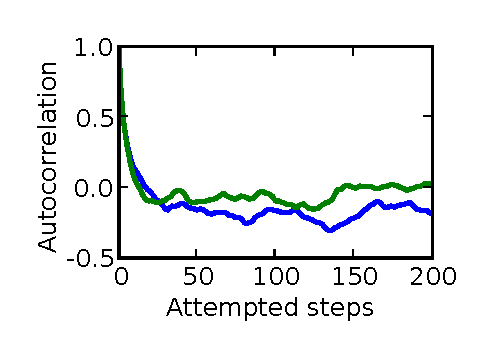
\includegraphics{autocorr}
\end{center}
\caption[Example autocorrelation functions]{Shown are autocorrelation functions functions for the cost (blue) and the logarithm of a particular parameter (green) in an ensemble built for the small JAK-STAT example model (Section~\ref{sec:user:example}). The correlation time for both is about 25 steps, suggesting that parameter sets 25 steps apart are statistically independent.\label{fig:user:autocorr}}
\end{figure}

There are several ways to assess convergence.
Most thorough (but computationally expensive) is to start several ensembles from very different initial parameters and see that they give identical answers for your predictions.

Given a single ensemble, one can check for convergence using the autocorrelation function of the cost and logarithms of the parameter values using \py{Ensembles.autocorrelation}.
Figure~\ref{fig:user:autocorr} shows example autocorrelation functions for a small model.
The number of independent samples in an ensemble is approximately the length of the ensemble divided by the \emph{longest} correlation time of any parameter in the ensemble.
Scaling arguments suggest that, for the default ensemble parameters, the number of steps in one autocorrelation time is at least the square of the number of parameters~\cite[Section 3.5.1]{bib:GutenkunstPhD}.

If the correlation time for your ensemble is much longer than the square of the number of parameters, your cost basin is probably substantially curved.
For advice on how to deal with this, see Section~\cite[Section 6.3]{bib:GutenkunstPhD}.

\subsubsection{Predicting from an Ensemble}

Once your ensemble has converged, you're ready to make predictions.
As a first step, you'll probably want to \emph{prune} your ensemble.
As mentioned previously, consecutive members of the ensemble are not independent, and it is independent samples that matter for predictions.
Once you've estimated the longest correlation time (\py{corr_steps}), the ensemble can be pruned simply by taking one member per correlation time: \py{ens_pruned = ens[::corr_steps]}.

To calculate uncertainties for any quantity over the ensemble, simply calculate its value for each member of your pruned ensemble and note the spread in values.
SloppyCell includes a few functions to make this easier in some common cases.
\py{Ensembles.ensemble_trajs} will integrate a \py{Network} for a fixed set of times over all members of an ensemble.
\py{Ensembles.traj_ensemble_quantiles} will calculate quantiles over those integrations, to show, for example, what the 95\% confidence bounds are on the trajectory prediction.
Similarly, \py{Ensembles.traj_ensemble_stats} will return trajectories containing the mean and standard deviation of each integration quantity over an ensemble.

\subsection{Plotting}

SloppyCell's plotting functionality is built upon matplotlib~\cite{bib:Hunter2007}, also known as \py{pylab}; a nice tutorial is available at \url{http://matplotlib.sourceforge.net/tutorial.html}.
SloppyCell's \py{Plotting} module adds several routines that are convenient for analyzing fits, ensembles, and Hessians.
For example, Figure~\ref{fig:user:model_results} shows a plot of the best fit for our example model (Section~\ref{sec:user:example}) with no additional tweaking.

\subsection{KeyedLists}
Numerical algorithms are generally designed to work with arrays of values, while users don't want to remember which parameter was number 97.
To solve both issues, SloppyCell uses a custom data type called a \py{KeyedList} which has properties of both Python lists and dictionaries.
Like a normal list, values can be accesses using \py{[<index>]} notation.
Additionally, each entry is associated with a key, so that values can be added and accessed using \py{get} and \py{set} methods like a Python dictionary.

\subsection{Input and Output \label{sec:user:IO}}

SloppyCell's \py{IO} module includes several functions to facilitate import and export of useful representations of \py{Network}s.

\begin{figure}
\begin{center}
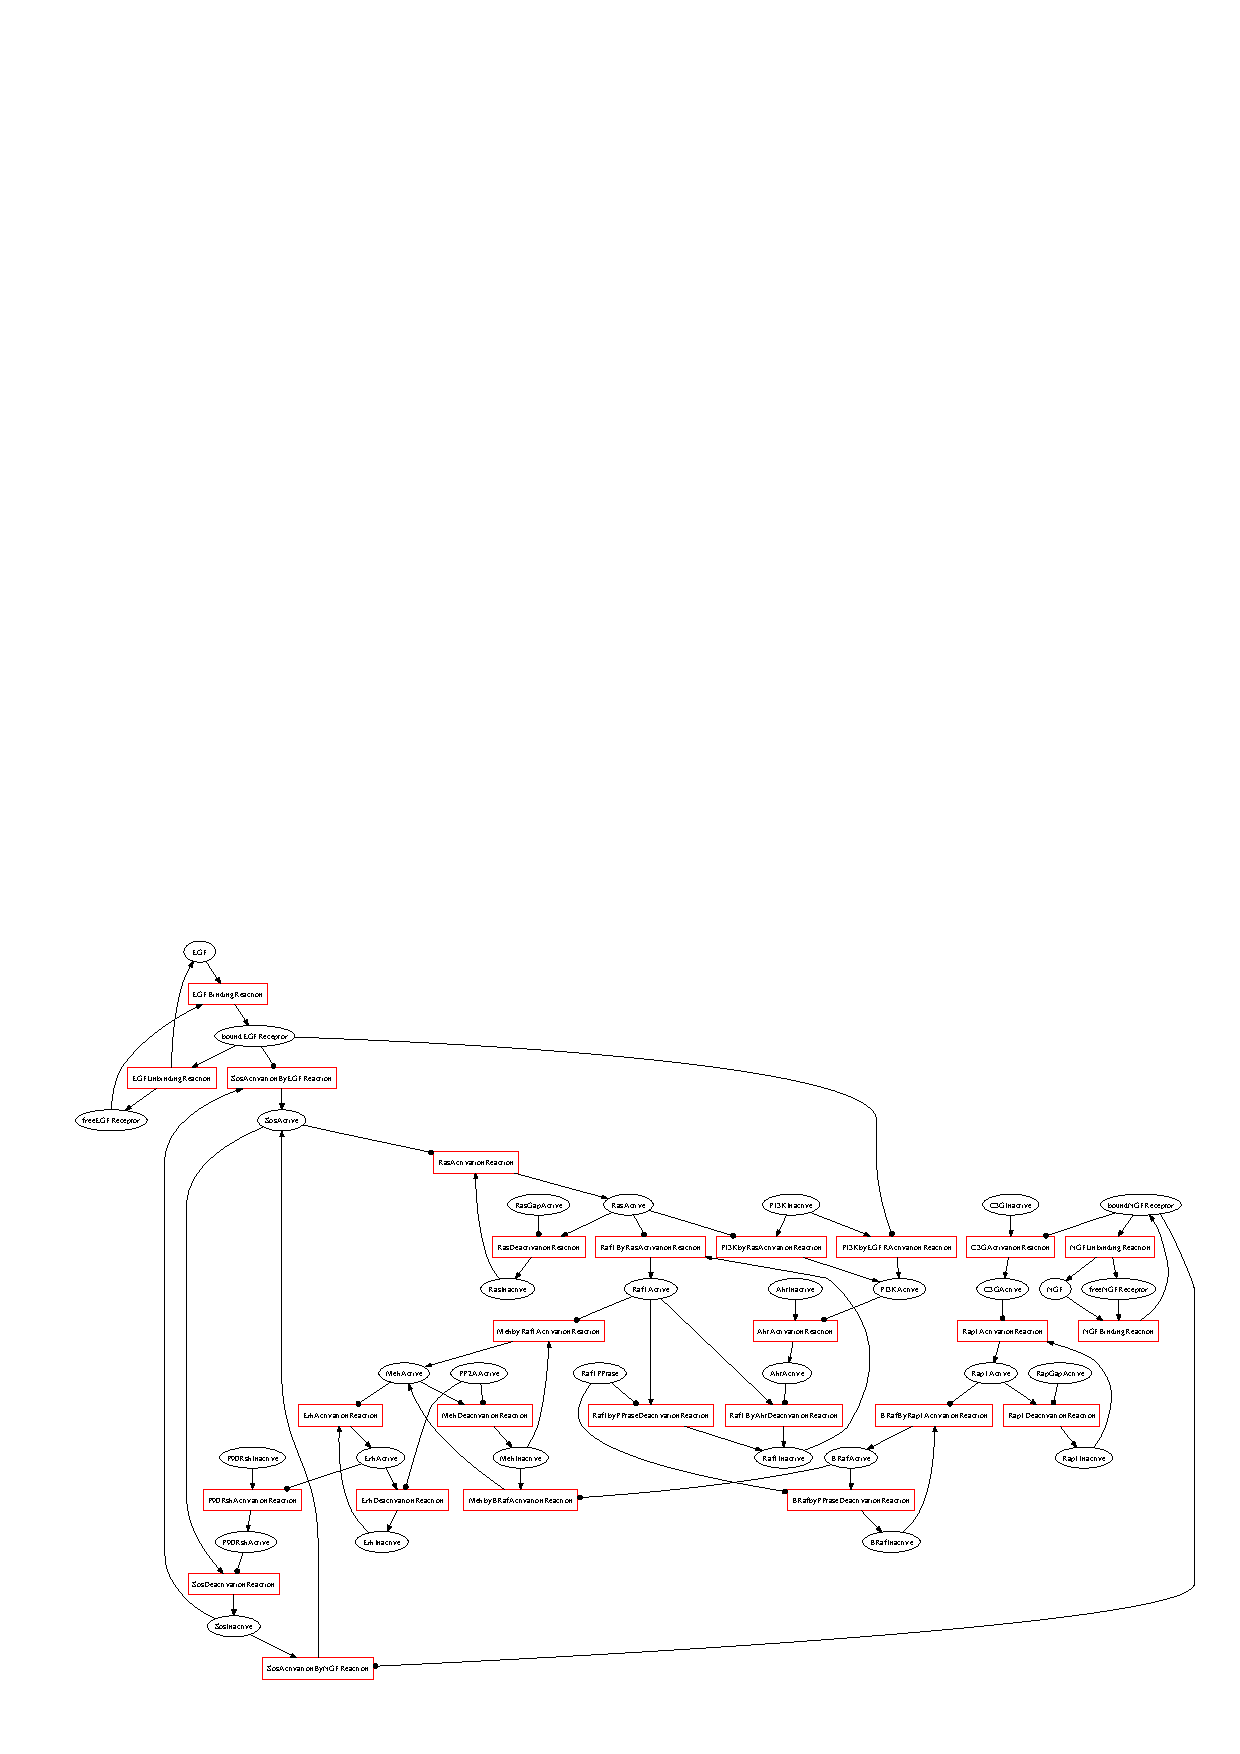
\includegraphics[width=\textwidth]{EGFstim100}
\end{center}
\caption[Automatically generated network diagram for G protein model]{Shown is a SloppyCell-generated network diagram for the growth-factor-signaling model of Brown et al.~\cite{bib:Brown2004}. Black ovals denote species and red boxes denote reactions between them.\label{fig:user:dot}}
\end{figure}

\py{IO.from_SBML_file} and \py{IO.to_SBML_file} allow importing and exporting of SBML files. (Note that SloppyCell will not preserve annotations of an SBML network that has been imported.)
\py{IO.net_DOT_file} generates \shell{dot} files which can be fed to Graphviz (\url{http://www.graphviz.org/}) to generate basic network diagrams as seen in Figure~\ref{fig:user:dot}.
Finally, \py{IO.eqns_TeX_file} will export a \shell{tex} file that can be used with \LaTeX to generate nicely-formatted equations. These are useful both for inclusion in publications and for debugging models.

\subsection{Miscellaneous Utilities}

To conveniently save results for future analysis, you can use \py{Utility.save} and \py{Utility.load}.
Note that these rely on Python's binary `pickle' format, so there is a slight danger that upgrades to Python or SloppyCell will render them unreadable. For more robust but less space-efficient saving, dump results to text files using, for example, \py{scipy.io.write_array}.

\subsection{Parallelization\label{sec:user:parallel}}

SloppyCell implements a relatively simple parallelization paradigm~\cite{bib:Myers2007} over MPI, using the PyPar (\url{http://sourceforge.net/projects/pypar/}) interface.
Two major tasks have been parallelized.
(1) If evaluating the cost of a \py{Model} involves integrating several \py{Network}s, those integrations can be spread across several processors.
(2) In \py{Dynamics.integrate_sensitivity}, the integrations for different parameters can be distributed across processors.
Parallel execution is enabled by a simple import:
\begin{lstlisting}
import SloppyCell.ReactionNetworks.RunInParallel as Par.
\end{lstlisting}
Anything in the script beyond this import will be run only by the master, who can send commands to the slaves. 
The slaves can be directly controlled using using methods in Par.
For example, \py{Par.statement_to_all_workers("print 'I am processor', my_rank")} will cause each processor to print a message giving its rank.

\section{Installation}\label{sec:user:install}

\subsection{Required Dependencies}
\begin{description}

\item[Python] version 2.4 or higher\\
 Available from \url{http://python.org/}.

\item[NumPy] version 1.0.2 or higher\\
 Available from \url{http://scipy.org/}

\item[SciPy] version 0.5.2 or higher\\
 Available from \url{http://scipy.org/}

\item[matplotlib] version 0.90.0 or higher\\
 Available from \url{http://matplotlib.sourceforge.net/}
\end{description}

\subsection{Optional Dependencies}

\begin{description}

\item[libSBML] version 2.3.4\\
Available from \url{http://www.sbml.org/software/libsbml/}.\\
If libSBML is installed, SloppyCell will be able read and write files encoded in the Systems Biology Markup Language~\cite{bib:Hucka2003}. See section~\ref{sec:user:IO}.

\item[IPython]
Available from \url{http://ipython.scipy.org/}.\\
IPython is a dramatic improvement over the standard python shell and we highly recommended it for interactive work.

\item[C compiler]
For speed, SloppyCell by default generates C versions of the network equations, and this requires a C compiler. 
If a C compiler is not installed, SloppyCell will run with Python versions of the network equations, which may be up to a factor of 30 slower. 
This capability has been tested only with the compiler \filename{gcc}, but it should work with others.

\item[Pypar]
Available from \url{http://sourceforge.net/projects/pypar/}.\\
With Pypar installed, SloppyCell can run several common calculations in parallel over MPI. See section~\ref{sec:user:parallel}
(As of August 21, 2007 the alpha version of Pypar 2.0 is required for compatibility with NumPy.)

%\item[\LaTeX]
%Available from \url{http://www.latex-project.org/}.\\
%\LaTeX is a document preparation system that is heavily used in the physical sciences. It handles mathematics beautifully, and SloppyCell can output \filename{.tex} files containing the equations defining a network. This is quite useful for debugging models. See section~\ref{sec:SCuser:LaTeX} for an example.

%\item[Graphviz]
%Available from \url{http://www.graphviz.org/}.\\
%SloppyCell can generate \filename{.dot} files specifying network diagrams which can be visualized using Graphviz. See section~\ref{sec:SCuser:dot} for an example.
\end{description}

\subsection{On Linux}
Installation on a Linux system should be straightforward, as Linux machines are generally well-equipped with the proper compilers.

\begin{enumerate}
\item Install the required dependencies
\item Unpack the tarball containing the SloppyCell code. (\shell{tar xzf SloppyCell-XXX.tar.gz})
\item Descend into the SloppyCell-XXX directory. (\shell{cd SloppyCell-XXX})
\item Run the installation script to build SloppyCell. (\shell{python setup.py build}).\\
Depending on your system, this may fail due to difficulties with Fortran compilation. The available Fortran compilers can be found with  \shell{python setup.py config_fc --help_fcompiler}, and if you contact us we can help with this step.
\item Run the installation script to install. (\shell{python setup.py install}).\\
If you prefer to use SloppyCell from the current directory rather than installing it elsewhere, use the \shell{--install-lib} option, \shell{python setup.py install --install-lib=..} . 
You will have to adjust your \shell{PYTHONPATH} environment variable to include the directory the SloppyCell directory is contained within. 
This installation option is particularly convenient for staying up-to-date with the CVS repository.
\end{enumerate}

\subsection{OS X}
Note that installation of libsbml with python bindings on Intel macs currently requires some work-arounds. Hopefully these will be resolved soon by the libsbml maintainers. If you're having difficulties, please contact us.

\subsubsection{Pre-built binary}
Binary \shell{mpkgs} are available from the Sourceforge download site.
These have been built against the framework builds of Python available from \url{http://www.python.org} on OS~X~10.4 (`Tiger').

\subsubsection{From source code}
Fortran compilers for OS X are available at  \url{http://hpc.sf.net}. Once you've installed 
such a compiler, follow the instructions for installing on Linux.

\subsection{Windows}
Installing \shell{gcc} on Windows requires some effort, but is highly suggested as it will dramatically speed up SloppyCell.

In our experience, the easiest way to get \shell{gcc} is to install \shell{MinGW}.
To install it, run \shell{MinGW-5.1.3.exe} from
\url{http://sourceforge.net/projects/mingw/}.
Tell the installer you want \shell{g77} and \shell{g++} in addition to the defaults.

Unfortunately, there is an issue with MinGW-5.1.3 that will cause compilation problems. To fix them, you will need to find \shell{libgcc.a} and run the following command:
\shell{ar dvs libgcc.a __main.o}~\cite{bib:SCuser:ar}.
On our test system \shell{libgcc.a} was in \shell{c:\\mingw\\lib\\gcc\\mingw32\\3.4.2}.

\subsubsection{Pre-built binary}
Pre-built binaries are available for Python 2.4 and Python 2.5.

\subsubsection{From source code}
Given that you installed \shell{g77} along during the MinGW install, you should be able to follow the Linux install instructions.

\subsection{Testing the Installation}\label{sec:test}
The SloppyCell source code includes a large package of test routines.
To access them: download and unpack \shell{SloppyCell-XXX.tar.gz} or \shell{SloppyCell-XXX.zip}, descend into the SloppyCell-XXX directory (\shell{cd SloppyCell-XXX}), and run \shell{cd Testing; python test.py}.
This will run an extensive series of tests, both with and without C-compilation.

\section{Troubleshooting}
\subsection{Failing Integrations}
Optimization or ensemble construction may explore regions of parameter space for which the model equations become very difficult to integrate, leading to many \py{daeint} exceptions being raised.
One possible solution is to check the `typical' values that are being assumed for each variable, accessible via \py{net.get_var_typical_vals()}.
These are used to help set the absolute tolerances of the integrations, and if they are very different from the values the variable actually attains, the inconsistency can cause problems.
The solution is then to set them to more reasonable values using \py{net.set_var_typical_val(<variable id>, <value>)}.

\bibliographystyle{../plos}
\bibliography{../bibliography}

\end{document}
